\chapter{Results}
\label{chapter:results}


\section{Q-Learning}
In the next figures the values predicted from Q are presented. As it can be noticed the optimal policy is as follows. The game allows the picker to move LEFT from first stack and move RIGHT from last stack (\textbf{e.g.} If the picker points to the first stack and chooses to move LEFT, then the picker will point to the last stack). In fig. \ref{fig:fa} the picker points to the second stack so the optimal action will be to move RIGHT. As we can see the value for the RIGHT-action is bigger than the other values. In fig. \ref{fig:fb} the agent has only one move to finish the game, in optimal conditions. Again, if we look at which value is greater than the others we can see that DOWN appears to be 100 which is exactly the value of the reward received when an episode is finished. Fig. \ref{fig:fc} presents the initial state of the game, just as expected the game should begin with the picking for the first time of a disk and that is exactly what Q-Learning is doing.

Another important aspect is that the values for actions corresponding to a state \textbf{s} are close. Why? This happens because the game has a static environment and there is no negative reward, thus whatever happens, the agent will always lose or it will be forced to play until the game is finished. The agent can never loose.

\begin{figure}[hp]
\centering
\minipage{0.32\textwidth}
  \frame{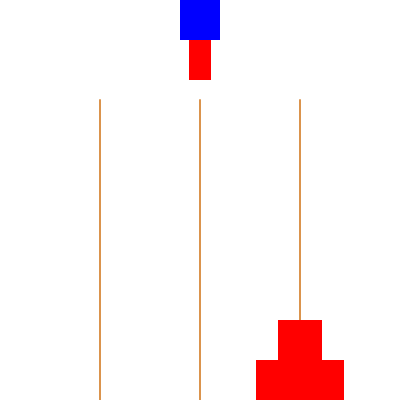
\includegraphics[width=\linewidth]{src/img/results/50}}
  \caption{\newline UP = 90,6534\newline DOWN = 86,8787\newline LEFT = 89,1867\newline RIGHT = 94,2824}\label{fig:fa}
\endminipage\hfill
\minipage{0.32\textwidth}
  \frame{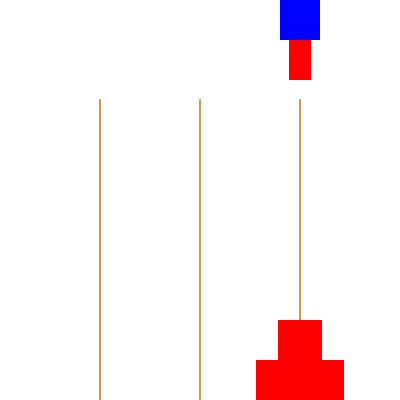
\includegraphics[width=\linewidth]{src/img/results/85}}
  \caption{\newline UP = 97,6530\newline DOWN = 100,0000\newline LEFT = 93,8538\newline RIGHT = 92,5261}\label{fig:fb}
\endminipage\hfill
\minipage{0.32\textwidth}%
  \frame{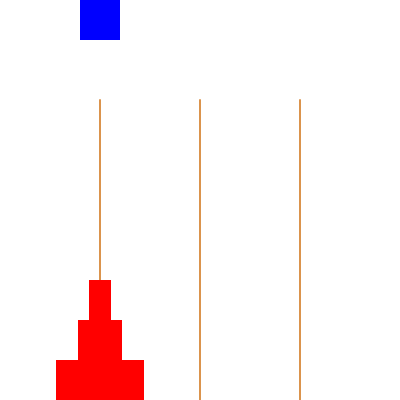
\includegraphics[width=\linewidth]{src/img/results/155}}
   \caption{\newline UP = 26,3520\newline DOWN = 23,8452\newline LEFT = 23,8897\newline RIGHT = 22,8827}\label{fig:fc}
 
\endminipage
\end{figure}

\newpage

\section{Regression with deep-learning and complex model}
In the last chapter we discussed the composition of the model. We stated that the last layer is formed of 100 neurons. Sometimes, neural networks are not as easy as we imagine to implement. Even if we have a big dataset, or even if we alter data in a way that we think it might work for the sake of generalization, bad things happen. As we can see from the figures, the network is doing very well at learning samples from the training dataset. It is worth mentioning that one epoch is equivalent to learning the train dataset once and get the error for forwarding the test dataset over the network. Also, to make a parallel, notice that the output values are normalized to the 0-1 range. Now, we can return to the graph and see that the training error behaves as we expect it to and yes, it is decreasing. However, the test error is not behaving mathematically as shown in figure \ref{fig:traintest}. This brings into question the validity of the model. One must observe that the slope of the train-line between the first epoch and the second epoch is steeper, which means that after only one epoch the network over learned the train-dataset and that is one reason for not being predicted well on the test-dataset. In either case, one can state that the model with 50 neurons is an improvement as opposed to the one with 100 neurons. From this we conclude that if the model is too complex, the network could run into the overfitting phenomenon.
\begin{figure}[h]
	\begin{center}
		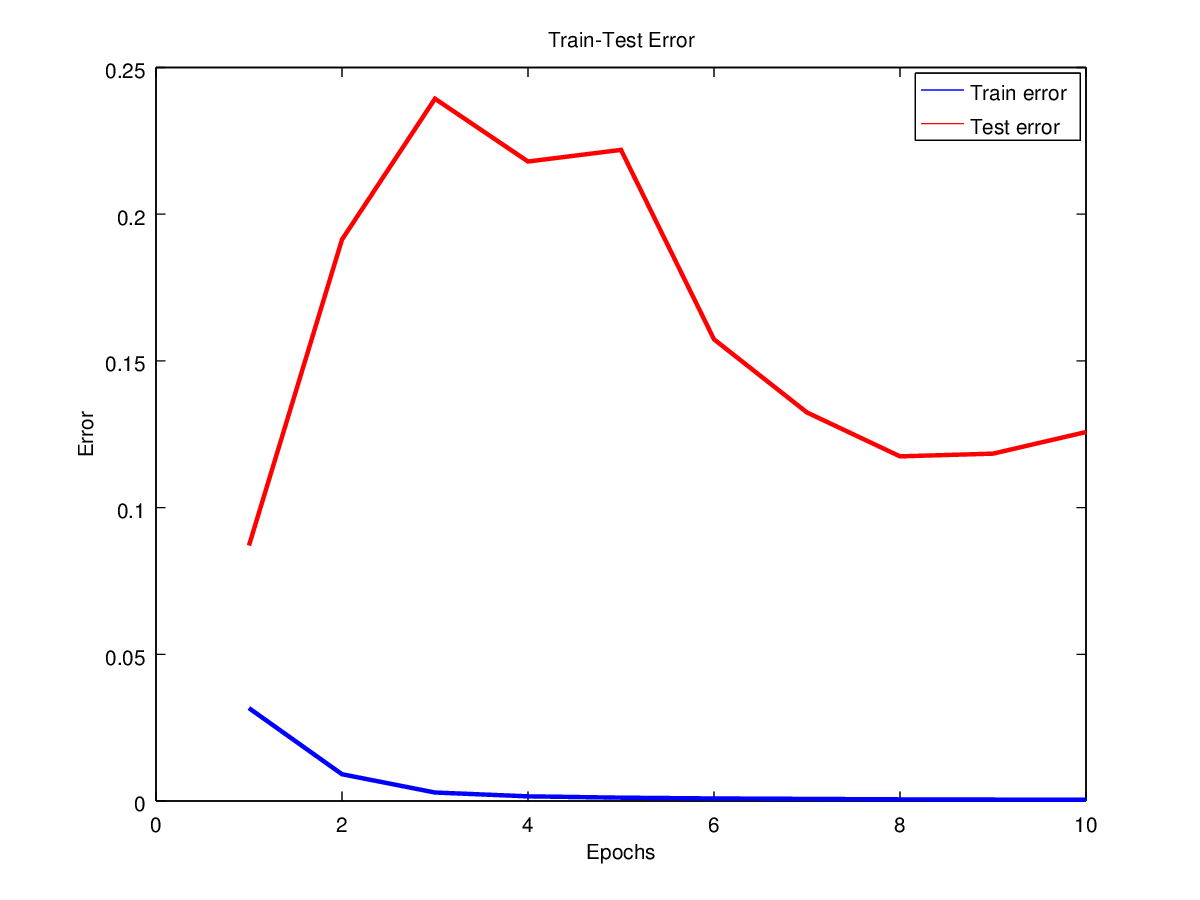
\includegraphics[width=209px,height=157px]{src/img/results/train-test-100}
		\caption{Last hidden fully connected layer has 100 neurons} \label{fig:50tt}
    \end{center}
\end{figure}
~\\
\begin{figure}[h]
	\begin{center}
		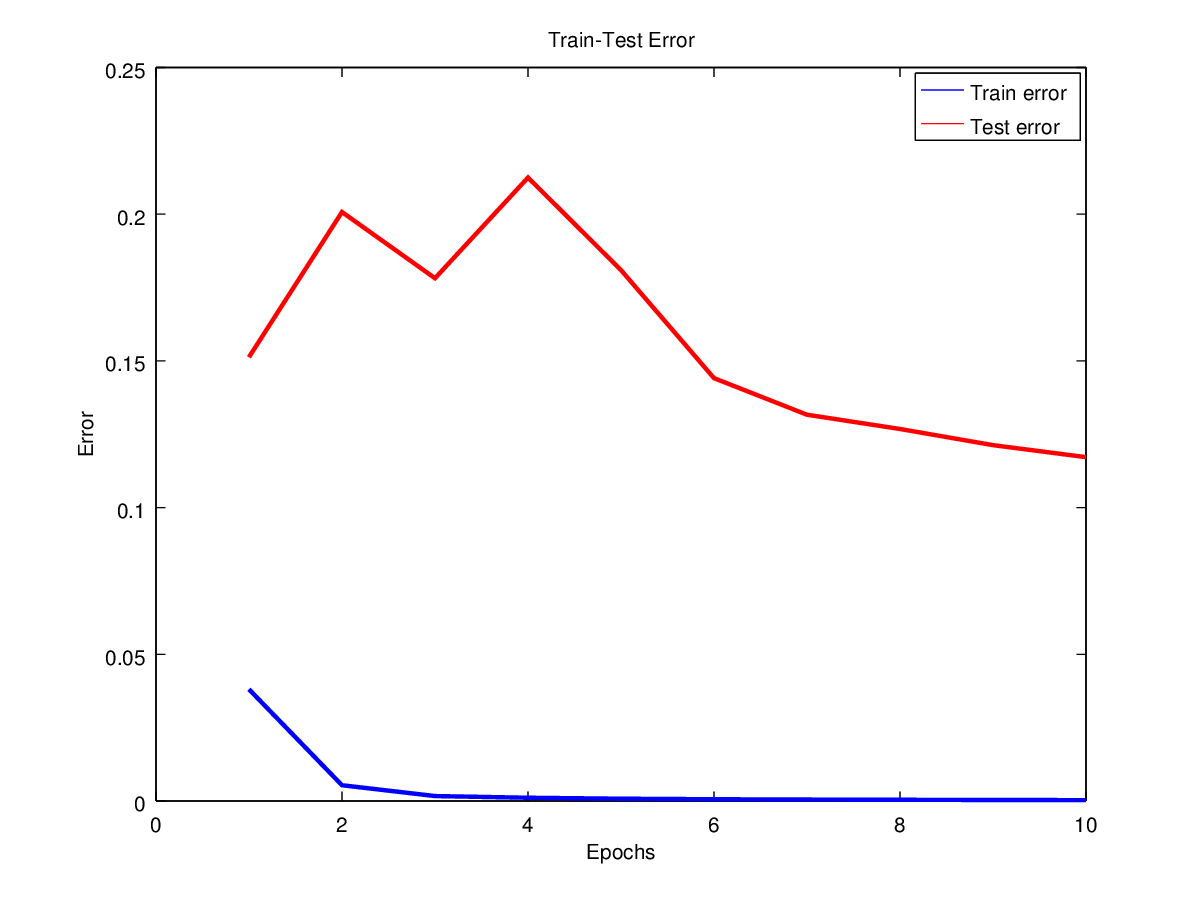
\includegraphics[width=209px,height=157px]{src/img/results/train-test-50}
		\caption{Last hidden fully connected layer has 50 neurons} \label{fig:100tt}
    \end{center}
\end{figure}

\section{Classification with deep-learning and complex model}

For updating weights in combination with backpropagation, SGD was used with learning rate $\alpha = 10^{-3}$. The train and testing have been done for 10 epochs and the average accuracy computed during the 10 epochs is approximately $33\%$. The dataset used is the same from regression, 10,000 pictures created from 160 pictures with noise added and color changed. Once again, the experiment showed unsatisfactory results. Transforming qlearning learned values to labels resulted in having unequal number of samples per class. This affects the network to learn more how a picture of class \textbf{c} looks and of course, in not learning the samples for the other classes. The graphic below gives the plot of the accuracy on both, train and test datasets.

\begin{figure}[h]
	\begin{center}
		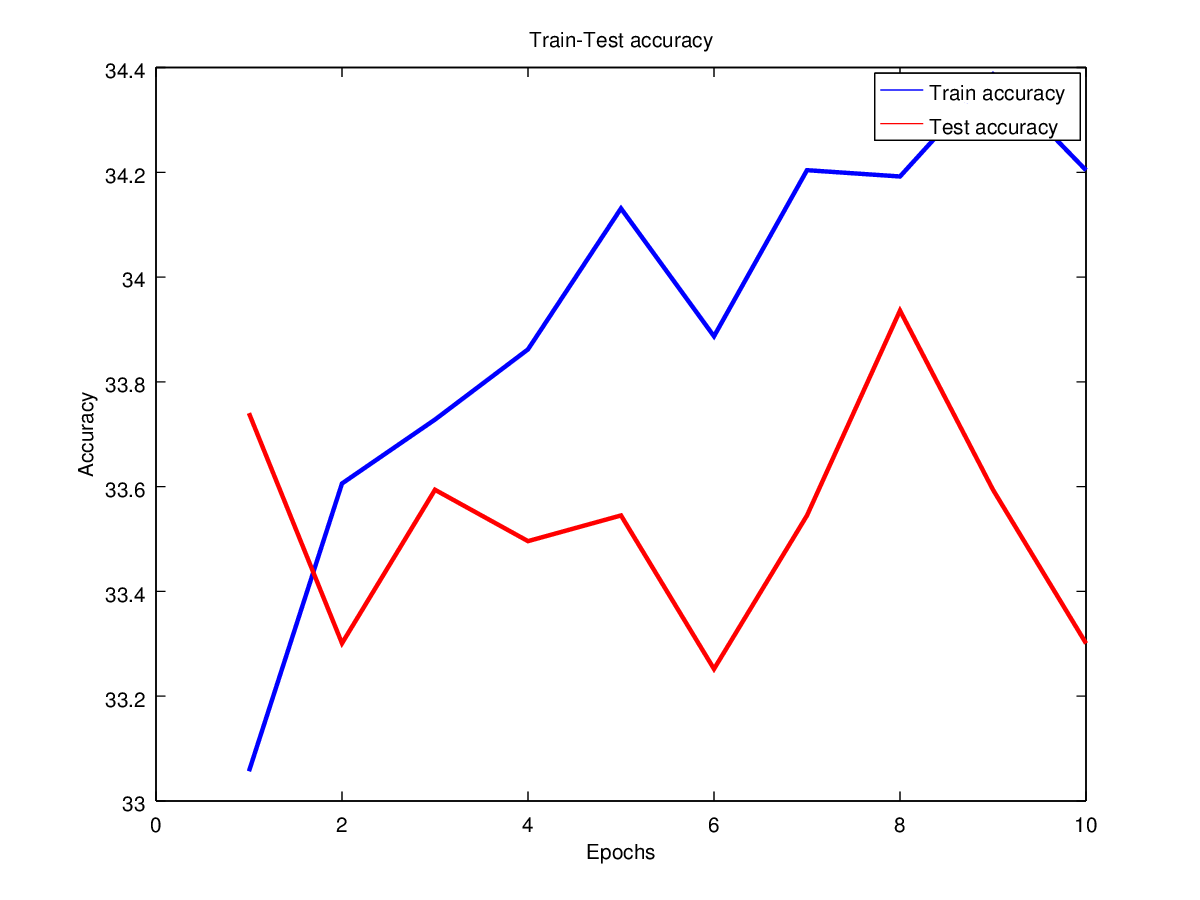
\includegraphics[width=209px,height=157px]{src/img/results/train-test-classif}
		\caption{Train-Test accuracy - classification} \label{fig:100tt}
    \end{center}
\end{figure}


\section{Regression with deep-learning and simple model}
Once again we used SGD with learning rate equals to 0.05. The train and testing has been done 10 epochs. The dataset used is the one with noise and color changed with 10,000 samples. This time, reducing the complexity of the network brings improvement in the results showed by the graphic below. After each epoch, the system is learning and this lead to a decreasing of both errors, for training and testing. While simple model can not learn to predict neither values they have seen nor new samples, complex model may learn very well examples and become incapable to predict for new samples. Both cases of anomalies lead to a neural network that could not be used for predicting anything. The main target is to have an agents that could do very well on unseen samples.
\newpage
\begin{figure}[h]
	\begin{center}
		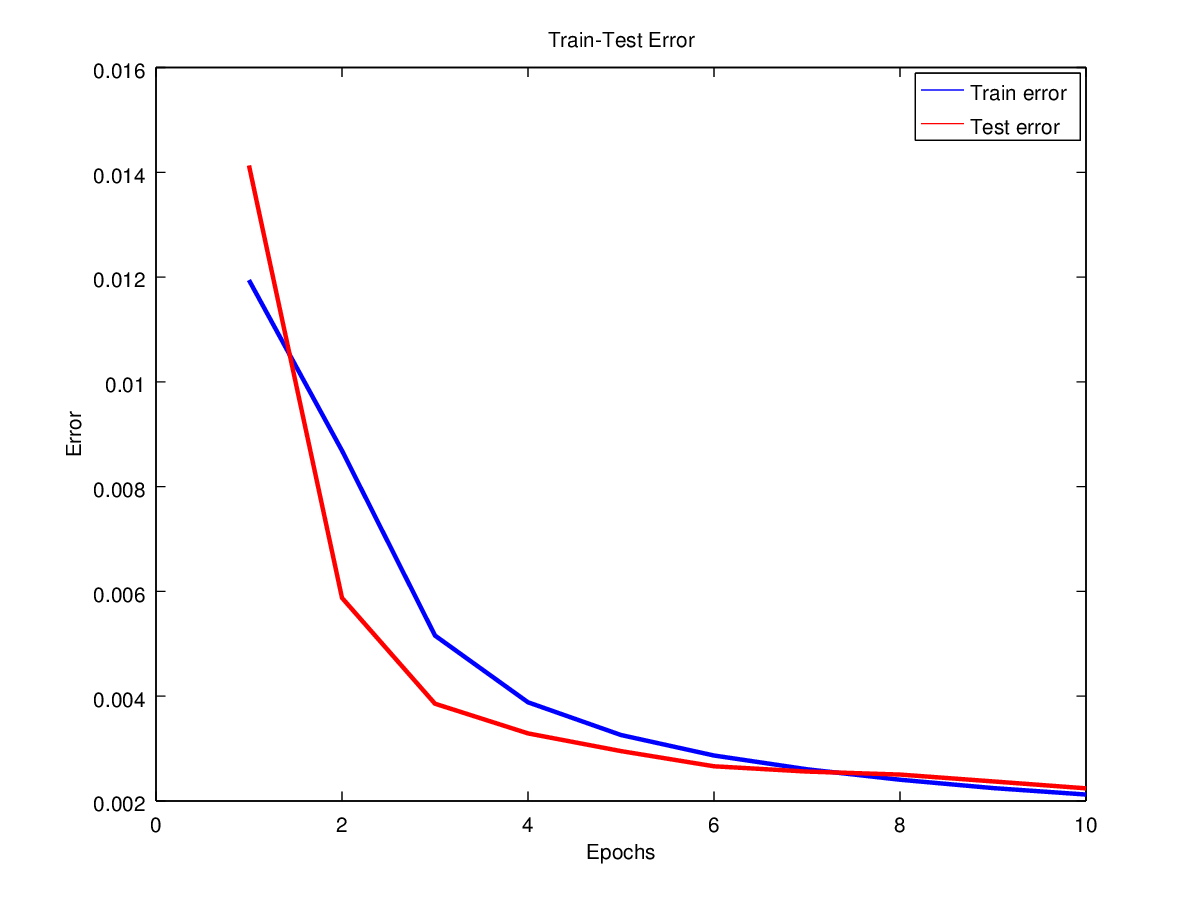
\includegraphics[width=209px,height=157px]{src/img/results/small-network}
		\caption{Train-Test error - simple model} \label{fig:100tt}
    \end{center}
\end{figure}




